\section{Prototypes}

\subsection{Cloud9}

We developed a \cnine prototype on top of the \klee~\cite{klee} symbolic execution engine.  The prototype has 7 \kloc.
%
The \klee modifications to support the symbolic OS abstractions amount to roughly 2 \kloc, while the rest consists of the POSIX model built on top of the abstractions.

\subsection{Chef}

We used \chef to generate symbolic execution engines for Python~(\S\ref{sec:python}) and Lua~(\S\ref{sec:lua}). Table~\ref{tab:pychanges} summarizes the effort to set up the two interpreters for \chef.  The necessary changes to the interpreter amount to 321 lines of code for Python and 277 for Lua.
%
The total developer time was 5 person-days for Python and 3 person-days for Lua, which is orders of magnitude smaller than the effort required for building a complete symbolic execution engine from scratch.  

\begin{table}
\centering
\small
\begin{tabular}{|@{\hspace*{4pt}}l@{\hspace*{4pt}}|@{\hspace*{4pt}}r@{\hspace*{4pt}}|@{\hspace*{4pt}}r@{\hspace*{4pt}}|}
\hline
\textbf{Component} & \textbf{Python} & \textbf{Lua}\\
\hline
Interpreter core size (C LoC) & 427,435 & 14,553 \\
\hline
\hline
HLPC instrumentation (C LoC) & 47 (0.01\%) & 44 (0.30\%) \\
Sym. optimizations (C LoC) & 274 (0.06\%) & 233 (1.58\%) \\
\hline
Native extensions (C LoC) & 1,320 (0.31\%) & 154 (1.06\%) \\
Test library (Python/Lua LoC) & 103 & 87 \\
\hline
\hline
Developer time (person-days) & 5 & 3 \\
\hline
\end{tabular}
\caption{Summary of the effort required to support Python and Lua in \chef.  The first row is the interpreter size without the standard language library. The next two rows are changes in the interpreter core, while the following two constitute the symbolic test library.  The last item indicates total developer effort.}
\label{tab:pychanges}
\end{table}

\subsubsection{Symbolic Execution Engine for Python}
\label{sec:python}

\paragraph{Interpreter Instrumentation}

We instrumented the CPython interpreter 2.7.3 for use with \chef, according to the guidelines presented in~\S\ref{sec:recipe}.

Python programs are composed of modules, corresponding to Python source files.  Each source file is compiled into an interpreter-specific bytecode format, i.e., each source statement is translated into one or more lower-level primitive instructions.  The instructions are grouped into blocks, corresponding to a single loop nesting, function, method, class, or global module definition.
%
We define an \hlpc as the concatenation of the unique block address of the top frame on the stack and the current instruction offset inside the block. We instrumented the Python interpreter to pass this program location to \chef; this required adding less than 50 LoC to the main interpreter loop.

We performed several optimizations on the Python interpreter: we neutralized the hash functions of strings and integers, which are the most common objects; we concretized the memory sizes passed to the garbage-collected memory allocator; and we eliminated interning for small integers and strings.    
%
Most optimizations involved only adding preprocessor directives for conditional compilation of blocks of code.
%
We gathered the optimizations under a new \codebit{--with-symbex} flag of the interpreter's \codebit{./configure} script.

\paragraph{Symbolic Tests}

To validate the usefulness of the resulting symbolic execution engine, we use it as a test case generation tool.  To this end, we implemented a symbolic test library as a separate Python package, used both inside the guest virtual machine, and outside, during test replay.
%
Figure~\ref{fig:sample-test} is an example of a symbolic test class for the \codebit{argparse} command-line interface generator. It sets up a total of 12 symbolic characters of input: two 3-character symbolic arguments to configure the command-line parser plus another two to exercise the parsing functionality.

The test class derives from the library's \codebit{SymbolicTest} class, which provides two methods to be overridden: \codebit{setUp}, which is run once before the symbolic test starts, and \codebit{runTest}, which creates the symbolic input and can check properties.  The symbolic inputs are created by calling the \codebit{getString} and \codebit{getInt} methods in the \codebit{SymbolicTest} API.

\begin{figure}
  \centering
  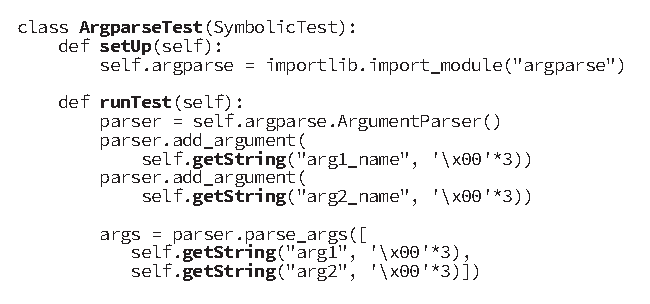
\includegraphics[width=3.2in]{figures/evaluation/symtest}
  \caption{The symbolic test used to exercise the functionality of the Python \codebit{argparse} package.}
  \label{fig:sample-test}
\end{figure}

A symbolic test is executed by a symbolic test runner, which is also part of the library.  The runner can work in either symbolic or replay mode. 
%
In \emph{symbolic mode}, the runner executes inside the guest virtual machine.  It creates a single instance of the test class, whose \codebit{getString} and \codebit{getInt} methods create corresponding Python objects and invoke the \codebit{make\_symbolic} call to mark their memory buffers as symbolic.
%
In \emph{replay mode}, the runner creates one instance of the test class for each test case created by \chef. The \codebit{getString} and \codebit{getInt} methods return the concrete input assignment of the test case.


\subsubsection{Symbolic Execution Engine for Lua}
\label{sec:lua}

Lua is a lightweight scripting language mainly used as an interpreter library to add scripting capabilities to software written in other languages. However, it also has a standalone interpreter and several Lua-only projects exist. We generated a symbolic execution engine for Lua based on version 5.2.2 of the Lua interpreter.

\paragraph{Interpreter Instrumentation}

Similar to Python, Lua programs are composed of one or more Lua source files, compiled into a bytecode format.  The code is compiled into a set of functions that operate on a global stack of values.  Each function is composed of a sequence of bytecode instructions, where each instruction is defined by an offset, opcode, and parameters.
%
We construct the \hlpc as the concatenation of the unique address of the function in the top frame and the current instruction offset being executed.  The instrumentation amounts to less than 50 LoC added to the interpreter loop.

We optimized the Lua interpreter for symbolic execution by eliminating string interning.  In addition, we configured the interpreter to use integer numbers instead of the default floating point, for which S2E does not support symbolic expressions.  This change was easy, because it was available as a macro definition in the interpreter's configuration header.

%%%%%%%%%%%%%%%%%%%%%%%%%%%%%%%%%%%%%%%%%%%%%%%%%%%%%%%%%%%%%%%%%%%%%%%%%%%%%%%%

\section{Experimental Setup and Testing Targets}

\subsection{Running Low-level Systems with Cloud9}



\subsection{Targeting Python and Lua Packages with Chef}

All reported \chef experiments were performed on a 48-core 2.3 GHz AMD Opteron 6176 machine with 512 GB of RAM, running Ubuntu 12.04. Each \chef invocation ran on 1 CPU core and used up to 8 GB of RAM on average.

\paragraph{Testing Targets}

\begin{table*}[!ht]
\centering
\footnotesize
\begin{tabular}{@{\hspace*{5pt}}l@{\hspace*{11pt}}r@{\hspace*{11pt}}l@{\hspace*{11pt}}l|r|c|c@{\hspace*{5pt}}}
\textbf{Package} & \textbf{LOC} & \textbf{Type} & \textbf{Description} & \textbf{Coverable LOC} & \textbf{Exceptions} & \textbf{Hangs}\\
\hline
\rule{0pt}{12pt}\textbf{Python} & & & & & \\
argparse$^{*}$ & 1,466 & System & Command-line interface & 1,174 & 4 / 0 & --- \\
ConfigParser$^{*}$ & 451 & System & Configuration file parser & 145 & 1 / 0 & --- \\
%
HTMLParser$^{*}$ & 623 & Web & HTML parser & 582 & 1 / 0 & --- \\
simplejson 3.10 & 1,087 & Web & JSON format parser & 315 & 2 / 0 & --- \\
%% webapp2 2.5.2 & 1,986 & Web & Web framework & & \\
%
unicodecsv 0.9.4 & 126 & Office & CSV file parser & 95 & 1 / 0 & --- \\
xlrd 0.9.2 & 7,241 & Office & Microsoft Excel reader & 4,914 & 5 / 4 & --- \\[2pt]
%
\hline
\rule{0pt}{12pt}\textbf{Lua} & & & & & & \\
cliargs 2.1-2 & 370 & System & Command-line interface & 273 & --- & --- \\
haml 0.2.0-1 & 984 & Web & HTML description markup & 775 & --- & --- \\
sb-JSON v2007 & 454 & Web & JSON format parser & 329 & --- & $\checkmark$ \\
markdown 0.32 & 1,057 & Web & Text-to-HTML conversion & 673 & --- & --- \\
moonscript 0.2.4-1 & 4,634 & System & Language that compiles to Lua & 3,577 & --- & --- \\[2pt]
%
\hline
\rule{0pt}{12pt}\textbf{TOTAL} & 18,493 & & & 12,852 & & \\
\end{tabular}
\caption{Summary of testing results for the Python and Lua packages
  used for evaluation. Items with (*) represent standard library
  packages.
  Exception numbers indicate total / undocumented exception types
  discovered.}
\label{tab:targets}
\end{table*}

We evaluated the symbolic execution engines for Python and Lua on 6 Python and 5 Lua packages, respectively, including system, web, and office libraries. In total, the tested code in these packages amounts to about $12.8$ KLOC.  We chose the latest versions of widely used packages from the Python standard library, the Python Package Index, and the Luarocks repository.  Whenever possible, we chose the pure interpreted implementation of the package over the native optimized one (e.g., the Python \codebit{simplejson} package). The first five columns of Table~\ref{tab:targets} summarize the package characteristics; LOC numbers were obtained with the \codebit{cloc} tool~\cite{cloc}.

The reported package sizes exclude libraries, native extension modules, and the packages' own test suites.
However, the packages ran in their unmodified form, using all the language features and libraries they were designed to use, including classes, built-in data structures (strings, lists, dictionaries), regular expressions, native extension modules, and reflection.  

All testing targets have a significant amount of their functionality written in the interpreted language itself; we avoided targets that are just simple wrappers around native extension modules (written in C or C++) in order to focus on the effectiveness of \chef at distilling high-level paths from low-level symbolic execution.  Nevertheless, we also included libraries that depend on native extension modules.  For instance, all the testing targets containing a lexing and parsing component use Python's standard regular expression library, which is implemented in C.
% The execution of parsers heavily depends on possible regular expression matches on input strings.
To thoroughly test these parsers, it is important to also symbolically execute the native regular expression library. For this, the binary symbolic execution capabilities of \chef are essential.

\paragraph{Methodology: Symbolic Tests}

For each package, we wrote a symbolic test that invokes the package's entry points with one or more symbolic strings.  
%The symbolic tests invoke the code under test in a generic manner without specific checks.  
Figure~\ref{fig:sample-test} in \S\ref{sec:symbolictests} is an example of such a symbolic test.

Each symbolic test ran for 30 minutes within \chef, after which we replayed the collected high-level tests on the host machine, in a vanilla Python/Lua environment, to confirm test results and measure line coverage.  To compensate for the randomness in the state selection strategies, we repeated each experiment 15 times.  In each graph we present average values and error margins as +/- one standard deviation.

For our experiments, we did not use explicit specifications, but relied on generic checks for finding common programming mistakes.  For both Python and Lua, we checked for interpreter crashes and potential hangs (infinite loops). 
For Python---which, unlike Lua, has an exception mechanism---we also flagged whenever a test case led to unspecified exceptions being thrown.
%
In general, one could find application-specific types of bugs by adding specifications in the form of assertions, as in normal unit tests.

\paragraph{Methodology: Coverage Measurement}

Line or statement coverage remains widely used, even though its meaningfulness as a metric for test quality is disputed. We measure and report line coverage to give a sense of what users can expect from a test suite generated fully automatically by a symbolic execution engine based on \chef.  For Python, we rely on the popular \codebit{coverage} package, and for Lua we use the \codebit{luacov} package.

Since our prototype only supports strings and integers as symbolic program inputs, we count only the lines of code that can be reached using such inputs. We report this number as ``coverable LOC'' in the fifth column of Table~\ref{tab:targets}, and use it in our experiments as a baseline for what such a symbolic execution engine could theoretically cover directly.  For example, for the \codebit{simplejson} library, this includes only code that decodes JSON-encoded strings, not code that takes a JSON object and encodes it into a string. Note that, in principle, such code could still be tested and covered by writing a more elaborate symbolic test that sets up a JSON object based on symbolic primitives~\cite{paas-testing}.

%%%%%%%%%%%%%%%%%%%%%%%%%%%%%%%%%%%%%%%%%%%%%%%%%%%%%%%%%%%%%%%%%%%%%%%%%%%%%%%%

\section{Test Suite Generation Effectiveness}

%%%%%%%%%%%%%%%%%%%%%%%%%%%%%%%%%%%%%%%%%%%%%%%%%%%%%%%%%%%%%%%%%%%%%%%%%%%%%%%%

\section{Bug Finding Effectiveness}

%%%%%%%%%%%%%%%%%%%%%%%%%%%%%%%%%%%%%%%%%%%%%%%%%%%%%%%%%%%%%%%%%%%%%%%%%%%%%%%%

\section{Scalability Analysis}

Discuss scalability of the Cloud9 parallelization algorithm.

Discuss overhead of Chef compared to hand-written engines.

%%% Local Variables: 
%%% mode: latex
%%% eval: (visual-line-mode)
%%% fill-column: 1000000
%%% TeX-master: "main"
%%% End:
